

    Neutrino physics is at the core of current high energy research. The standard model of particle physics explains many elements of the physical nature of our universe, though we now know that it does not cover everything. If neutrinos were to be described by the standard model they would be massless, but this was proved not to be the case when the Super-Kamiokande experiment observed neutrino flavour oscillations \textbf{find reference}. Neutrino research provided the first confirmation of the existence of physics beyond the standard model. \\

    Future, long-baseline,  neutrino experiments such as the Deep Underground Neutrino Experiment (DUNE) and Hyper-Kamiokande (Hyper-K) are hoping to investigate some of the most fundamental questions we are still asking: Why does the universe constist of matter, and not anti-matter? What is the neutrino mass heirarchy? \\

    Neutrino research is an extremely active field. Optimising the current and future detectors to maximise the accuracy of all interaction anaylses is a crucial step towards obtaining concrete answers to these questions.

\subsection{Neutrino interactions}

Due to the elusive nature of the neutrino, directly observing one in a detector isn't possible. It is therefore necessary to infer their existence from particles produced when they interact. Since this process relies upon the reconstruction capability of the experiment, purpose-built detectors have been constructed to maximise the efficiency of neutrino reconstruction. \\




\subsection{GENIE}

    GENIE is the world leading neutrino interaction generator. 

\subsection{Cross-sections}
    
    % Plan
    \begin{itemize}

        \item Why?
        
        \begin{itemize}

            \item Simulation
            \item GENIE

        \end{itemize}
        
        \item Historical
        \item Current knowledge
        \item Needs for future
        
        \begin{itemize}

            \item LArTPCs
            \item Statistics

        \end{itemize}

    \end{itemize}

    % Table
    \renewcommand{\arraystretch}{1.3}
\begin{center}
\begin{tabular}{lll}
    \textbf{Process} & & \textbf{No. Events} \\ 
    \hline\hline
    \multicolumn{3}{c}{\textit{\( \nu_{ \mu } \) Events }}\\
        CC 0 \( \pi \)                 & \( \nu_{ \mu } N \rightarrow \mu + Np \)                            & \textbf{3,551,830} \\
        CC 1 \( \pi^{ \pm } \)         & \( \nu_{ \mu } N \rightarrow \mu + nucleons +  1\pi^{ \pm } \)      & \textbf{1,161,610} \\
        CC \( \geq 2\pi^{ \pm } \)     & \( \nu_{ \mu } N \rightarrow \mu + nucleons + \geq 2\pi^{ \pm } \)  & 97,929 \\
        CC \( \geq 1\pi^{ 0 } \)       & \( \nu_{ \mu } N \rightarrow \mu + nucleons + \geq 1\pi^{ 0 } \)    & 497,963 \\
        \hline        
        NC 0 \( \pi \)                 & \( \nu_{ \mu } N \rightarrow nucleons \)                            & 1,371,070 \\
        NC 1 \( \pi^{ \pm } \)         & \( \nu_{ \mu } N \rightarrow nucleons +  1\pi^{ \pm } \)            & 260,924 \\
        NC \( \geq 2\pi^{ \pm } \)     & \( \nu_{ \mu } N \rightarrow nucleons + \geq 2\pi^{ \pm } \)        & 31,940 \\
        NC \( \geq 1\pi^{ 0 } \)       & \( \nu_{ \mu } N \rightarrow nucleons + \geq 1\pi^{ 0 } \)          & 358,443 \\
        \hline\hline
        \multicolumn{2}{l} {Total \( \nu_{ \mu } \) \& \( \nu_{ e } \) events }                              & \textbf{7,251,948} \\
\end{tabular}
\end{center}

    
    %LArTPC
    \begin{figure}[h!]
        \center
        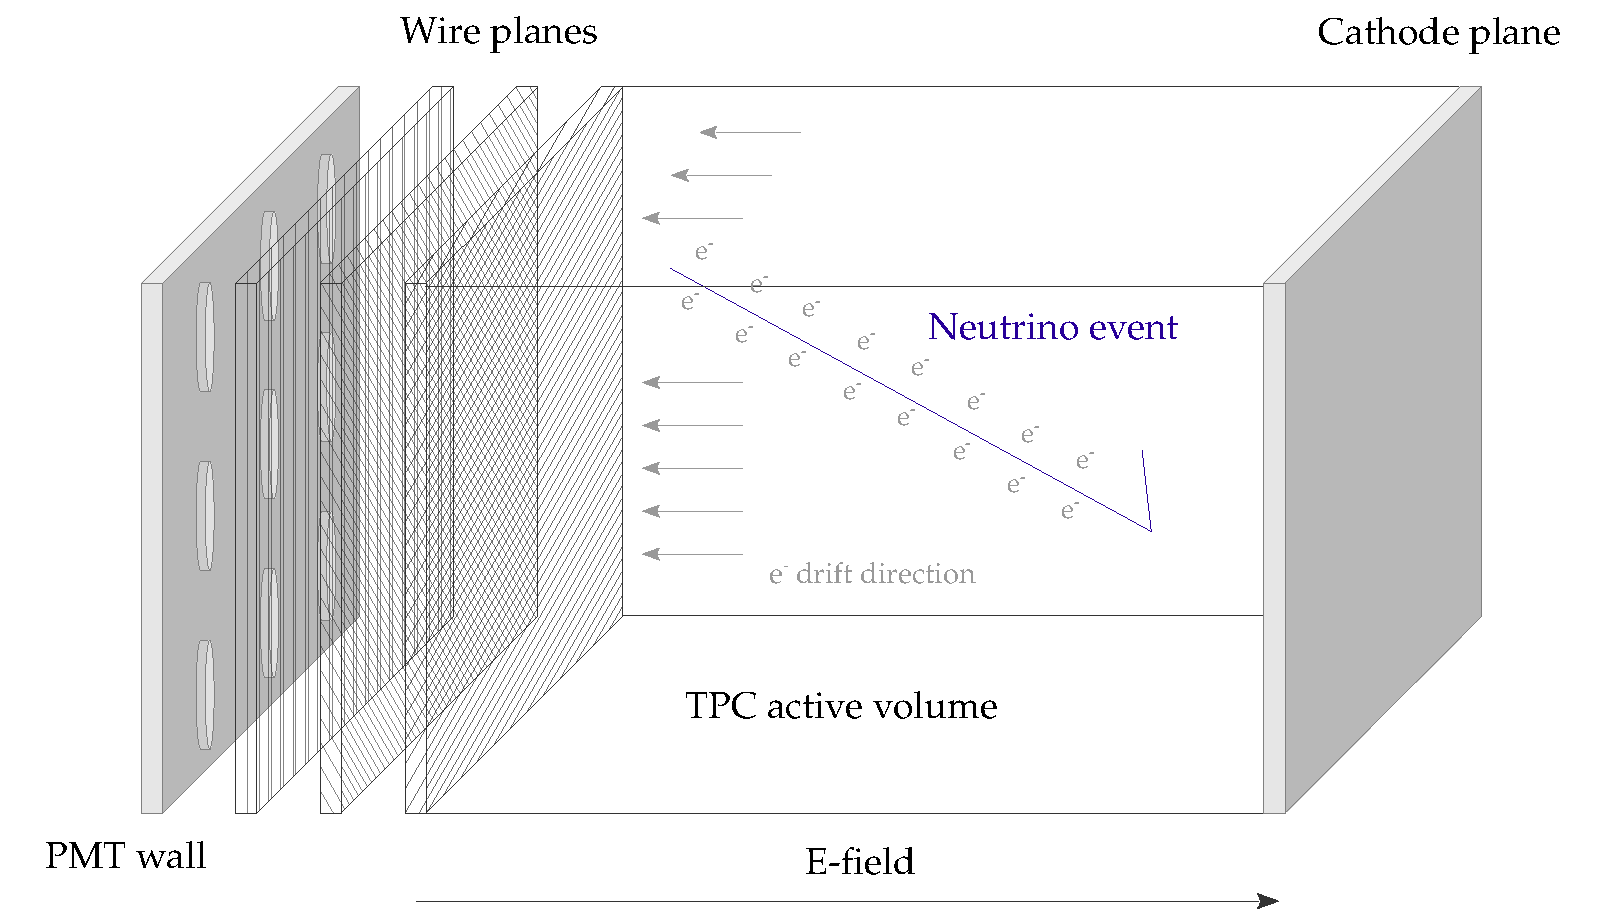
\includegraphics[width=\textwidth]{images/LArTPC.pdf}
    \end{figure}

\subsection{SBND}    

    % Plan
    \begin{itemize}

        \item LArTPC general functionality
        \item LArTPC resolution benefits
        \item Comparison with other detector materials
            \begin{itemize}
                \item Example event display?
            \end{itemize}
        \item SBND specifics

        \begin{itemize}

            \item Dimensions
            \item Beamline
            \item Flux
            \item Statistics

        \end{itemize}

        \item Cross-section precision capabilites

    \end{itemize}

\subsection{GENIE-Professor global fits}


\clearpage
